\documentclass[11pt,a4paper]{report}
\usepackage[margin=1in]{geometry}
\usepackage[T1]{fontenc}
\usepackage{lmodern}
\usepackage{hyperref}
\usepackage{booktabs}
\usepackage{longtable}
\usepackage{listings}
\usepackage{xcolor}
\usepackage{graphicx}
\usepackage{tikz}
\usetikzlibrary{shapes,arrows.meta,positioning,fit}

\hypersetup{colorlinks=true,linkcolor=blue,urlcolor=blue}

\lstdefinestyle{bash}{
  basicstyle=\ttfamily\small,
  breaklines=true,
  frame=single,
  backgroundcolor=\color{gray!8}
}

\title{CXR ELK Lab Manual\\
\large SW.12 --- logs (Elasticsearch + Kibana + Filebeat)\\
\large Connecting Claim Studio :3000 to Kibana}
\author{CXR Ops Lab --- \texttt{cxr-ops-lab}}
\date{2026-05-31}

\begin{document}
\maketitle
\begin{abstract}
Step-by-step lab for \textbf{SW.12 ELK}: every file added for log shipping, how the
\textbf{Claim Studio dashboard} on \textbf{:3000} produces Docker logs that Filebeat indexes,
and how \textbf{Kibana (:5601)} is where you search them. Contrasts with \textbf{Jaeger (:16686)} traces (SW.11)
and \textbf{Grafana (:3001)} metrics (SW.9--10). After you close the lab, ELK may stay stopped;
Jaeger remains useful for rehearsal \textbf{:8251}.
\end{abstract}
\tableofcontents
\newpage

\chapter{Where you view telemetry (three pillars)}

\begin{center}
\begin{tabular}{lllll}
\toprule
Signal & Tool & URL & Bootcamp SW & Web UI? \\
\midrule
Metrics & Prometheus & :9090 & SW.9 & API \\
Dashboards & \textbf{Grafana} & \textbf{:3001} & SW.10 & \textbf{Yes} \\
Traces & \textbf{Jaeger} & \textbf{:16686} & SW.11 & \textbf{Yes} \\
\textbf{Logs} & \textbf{Kibana} & \textbf{:5601} & \textbf{SW.12} & \textbf{Yes} \\
Log store & Elasticsearch & :9200 & SW.12 & API (no UI) \\
Shipper & Filebeat & (container) & SW.12 & \textbf{No UI} \\
\bottomrule
\end{tabular}
\end{center}

\noindent\textbf{Main CXR app (Claim Studio):} \url{http://localhost:3000/claim-studio} --- this is the
\textbf{product dashboard} you use to run analysis. It does \emph{not} embed Kibana or Jaeger; those are
\textbf{separate observability UIs} you open in other browser tabs when debugging.

\chapter{How :3000 Claim Studio connects to Kibana (highlight)}

\section{End-to-end path}

\begin{center}
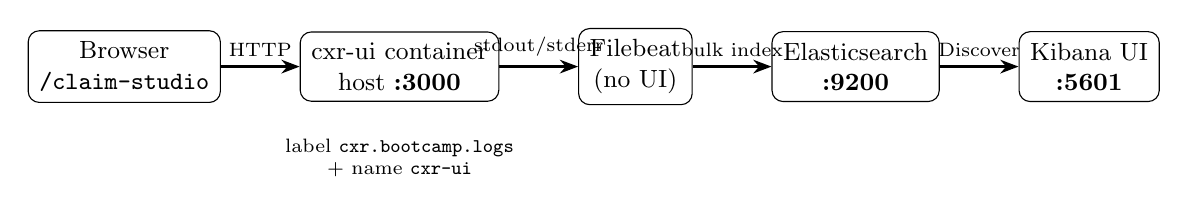
\begin{tikzpicture}[
  node distance=0.65cm and 0.5cm,
  box/.style={draw, rounded corners, minimum height=0.75cm, align=center, font=\small, inner sep=4pt},
  arr/.style={-{Stealth}, thick}
]
  \node[box] (br) {Browser\\\texttt{/claim-studio}};
  \node[box, right=1cm of br] (ui) {cxr-ui container\\host \textbf{:3000}};
  \node[box, right=1cm of ui] (fb) {Filebeat\\(no UI)};
  \node[box, right=1cm of fb] (es) {Elasticsearch\\\textbf{:9200}};
  \node[box, right=1cm of es] (kb) {Kibana UI\\\textbf{:5601}};
  \draw[arr] (br) -- node[above,font=\scriptsize]{HTTP} (ui);
  \draw[arr] (ui) -- node[above,font=\scriptsize]{stdout/stderr} (fb);
  \draw[arr] (fb) -- node[above,font=\scriptsize]{bulk index} (es);
  \draw[arr] (es) -- node[above,font=\scriptsize]{Discover} (kb);
  \node[below=0.35cm of ui, font=\scriptsize, align=center] {label \texttt{cxr.bootcamp.logs}\\
  + name \texttt{cxr-ui}};
\end{tikzpicture}
\end{center}

\section{What ``connects'' the main dashboard}

\begin{enumerate}
  \item \textbf{Compose CXR UI running} --- \texttt{./scripts/04-compose-up.sh} starts the \texttt{cxr-ui} service on \textbf{:3000}.
  \item \textbf{Label on the service} --- \texttt{compose.yaml} sets \texttt{cxr.bootcamp.logs: "true"} so Filebeat autodiscover selects the container.
  \item \textbf{ELK stack running} --- \texttt{./scripts/16-elk-up.sh} starts Elasticsearch, Kibana, Filebeat (\texttt{compose.elk.yaml}).
  \item \textbf{Filebeat config} --- \texttt{observe/elk/filebeat.yml} watches Docker via socket; matches container name \texttt{cxr-ui} or the label above; reads \texttt{/var/lib/docker/containers/.../*.log}.
  \item \textbf{User action on Claim Studio} --- page loads and \textbf{Run Analysis} write Next.js / server lines to the container log stream.
  \item \textbf{Indexing} --- Filebeat ships JSON events to Elasticsearch (indices like \texttt{filebeat-*}).
  \item \textbf{Kibana} --- Data view \texttt{filebeat-*}, \textbf{Discover}, filter e.g.\ \texttt{claim-studio}; screenshot for evidence.
\end{enumerate}

\section{What is \emph{not} wired (important)}

\begin{itemize}
  \item \textbf{Rehearsal :8251} (\texttt{npm run dev:rehearsal}) --- logs go to the \emph{host terminal}, not the \texttt{cxr-ui} Docker container. SW.12 evidence uses \textbf{:3000} Compose traffic unless you add a custom Filebeat input later.
  \item \textbf{Jaeger (SW.11)} --- traces from :8251 with \texttt{OTEL\_*}; does \emph{not} replace log search. Jaeger answers latency; Kibana answers ``what did the server print?''
  \item \textbf{Grafana (:3001)} --- metrics dashboards; not application log lines.
\end{itemize}

\section{Jaeger vs Elasticsearch (when ELK feels like overkill)}

For a \textbf{single-service} bootcamp app, running ELK every day is optional.
\begin{itemize}
  \item \textbf{Keep for the lab:} prove SW.12 (Discover screenshot + \texttt{evidence/SW12-elk-verify-2026-05-29.md}).
  \item \textbf{Then:} \texttt{docker compose -f compose.elk.yaml down} to free RAM; keep \texttt{07-observe-up.sh} + Jaeger for trace work on :8251.
  \item \textbf{Production pattern:} many teams run logs + traces + metrics; syllabus teaches all three.
\end{itemize}

\chapter{Step-by-step procedure}

\section{Step 1 --- Start Compose :3000 (log source)}
\begin{lstlisting}[style=bash]
cd cxr-ops-lab
./scripts/04-compose-up.sh
curl -sf http://localhost:3000 >/dev/null && echo "OK :3000"
\end{lstlisting}

\section{Step 2 --- Start ELK stack}
\begin{lstlisting}[style=bash]
./scripts/16-elk-up.sh
./scripts/16-elk-smoke.sh
\end{lstlisting}
Wait up to $\sim$60\,s after first start for Kibana to answer on \textbf{:5601}.

\section{Step 3 --- Golden path: Claim Studio $\rightarrow$ logs $\rightarrow$ Kibana}
\begin{enumerate}
  \item \url{http://localhost:3000/claim-studio}
  \item Click \textbf{Run Analysis} (or reload pages several times).
  \item Wait $\sim$30\,s for Filebeat to index new lines.
  \item \url{http://localhost:5601} $\rightarrow$ \textbf{Explore on my own} (skip Add integrations).
  \item \textbf{Stack Management $\rightarrow$ Data Views} $\rightarrow$ create \texttt{filebeat-*} (timestamp \texttt{@timestamp}).
  \item \textbf{Discover} $\rightarrow$ select data view (e.g.\ ``new CXR'') $\rightarrow$ time range \textbf{Last 24 hours} $\rightarrow$ refresh.
  \item Optional KQL: \texttt{claim-studio} or \texttt{analyze}.
  \item Screenshot for \texttt{evidence/SW12-kibana-discover-*.png}.
\end{enumerate}

\section{Step 4 --- Kibana UI tips}
\begin{itemize}
  \item Ignore \textbf{Security} sidebar (Alerts/Findings) on Home --- not required for this lab.
  \item Histogram brush zoom: \textbf{undo arrow} only appears right after brushing; otherwise click the \textbf{time range} picker $\rightarrow$ \textbf{Last 24 hours} $\rightarrow$ Update + refresh.
  \item Expect fields such as \texttt{agent.name: filebeat}, \texttt{container.id}, \texttt{@timestamp}.
\end{itemize}

\section{Step 5 --- Write evidence}
Edit \texttt{evidence/SW12-elk-verify-2026-05-29.md}: checkboxes for data view, Discover screenshot, golden path note.

\section{Step 6 --- Stop ELK (optional, after lab)}
\begin{lstlisting}[style=bash]
docker compose -f compose.elk.yaml down
\end{lstlisting}
Claim Studio on :3000 keeps working without ELK.

\chapter{Files created for SW.12 (full inventory)}

\begin{longtable}{@{}p{4.8cm}p{8.2cm}@{}}
\toprule
File & Purpose \\
\midrule
\endhead
\texttt{compose.elk.yaml} & Elasticsearch :9200, Kibana :5601, Filebeat; volume \texttt{elk\_es\_data} \\
\texttt{observe/elk/filebeat.yml} & Docker autodiscover $\rightarrow$ \texttt{cxr-ui} / label \texttt{cxr.bootcamp.logs} \\
\texttt{scripts/16-elk-up.sh} & \texttt{docker compose -f compose.elk.yaml up -d} \\
\texttt{scripts/16-elk-smoke.sh} & Health: ES, Kibana :5601, Filebeat running, \texttt{filebeat-*} index \\
\texttt{scripts/build-elk-manual-pdf.sh} & Builds this PDF from \texttt{CXR-ELK-LAB-MANUAL.tex} \\
\texttt{docs/CXR-ELK-LAB-MANUAL.md} & Markdown twin of this manual \\
\texttt{docs/CXR-ELK-LAB-MANUAL.tex} & LaTeX source for PDF \\
\texttt{docs/CXR-ELK-LAB-MANUAL.pdf} & Printable lab record (run build script) \\
\texttt{evidence/SW12-elk-verify-2026-05-29.md} & Verify checklist + agent smoke notes \\
\end{longtable}

\section{Files touched (not new)}

\begin{longtable}{@{}p{4.8cm}p{8.2cm}@{}}
\toprule
File & Change \\
\midrule
\endhead
\texttt{compose.yaml} & Label \texttt{cxr.bootcamp.logs: "true"} on \texttt{cxr-ui} service \\
\texttt{docs/OBSERVE-WIRING.md} & SW.12 URLs and commands \\
\texttt{docs/PLATFORM-SYLLABUS-MAP.md} & Maps SW.12 to ELK compose + manual \\
\end{longtable}

\section{Related observe stack (SW.9--11, separate compose)}

\begin{longtable}{@{}p{4.8cm}p{8.2cm}@{}}
\toprule
File & Role \\
\midrule
\endhead
\texttt{compose.observe.yaml} & Prometheus, Grafana, Jaeger, otel-collector \\
\texttt{compose.otel-link.yaml} & Optional: link Compose :3000 to collector for traces \\
\texttt{instrumentation.ts} + \texttt{register-otel-node.ts} & SW.11 traces (:8251 / optional :3000) \\
\texttt{docs/CXR-OTEL-LAB-MANUAL.pdf} & SW.11 trace lab (Jaeger, not logs) \\
\end{longtable}

\chapter{Port map (CXR lab)}

\begin{center}
\begin{tabular}{lll}
\toprule
Port & Service & Role in this manual \\
\midrule
3000 & Compose \texttt{cxr-ui} & \textbf{Claim Studio --- log source} \\
5601 & Kibana & \textbf{Log search UI} \\
9200 & Elasticsearch & Log index API \\
8251 & Rehearsal dev & Traces (SW.11), \emph{not} default log source \\
16686 & Jaeger & Traces UI (SW.11) \\
3001 & Grafana & Metrics dashboards (SW.10) \\
9090 & Prometheus & Metrics scrape (SW.9) \\
4318 & OTel collector & Trace ingest (no browser UI) \\
\bottomrule
\end{tabular}
\end{center}

\chapter{Implementation checklist (repeat on another machine)}

\begin{enumerate}
  \item Start \texttt{cxr-ui} on :3000 (\texttt{04-compose-up.sh}).
  \item Confirm label \texttt{cxr.bootcamp.logs} on the service in \texttt{compose.yaml}.
  \item Start ELK (\texttt{16-elk-up.sh}); run \texttt{16-elk-smoke.sh}.
  \item Generate traffic on Claim Studio (:3000).
  \item Kibana Discover on \texttt{filebeat-*}; save screenshot to \texttt{evidence/}.
  \item Optional: stop ELK; proceed syllabus \textbf{SW.14 Redis}.
\end{enumerate}

\chapter{Troubleshooting}

\begin{itemize}
  \item \textbf{No \texttt{filebeat-*} index} --- :3000 not up or no Claim Studio traffic; wait 30\,s; re-run \texttt{16-elk-smoke.sh}.
  \item \textbf{Kibana empty Discover} --- widen time range (Last 24 hours); clear KQL; refresh.
  \item \textbf{Only 6 docs in a 1h window} --- normal if traffic was brief; generate more :3000 loads.
  \item \textbf{Expected logs on :8251 dev} --- not shipped unless you extend Filebeat; use :3000 for SW.12.
  \item \textbf{Kibana slow first boot} --- allow $\sim$60\,s after \texttt{16-elk-up}.
\end{itemize}

\chapter{Study plan linkage}

\begin{center}
\begin{tabular}{ll}
\toprule
Item & Maps to \\
\midrule
Starter / post-starter electives & SW.12 logs \\
After SW.12 evidence & SW.14+ electives \\
Deferred & Phase 2 M1 C4 infill \\
\bottomrule
\end{tabular}
\end{center}

\chapter{Live adjustments (Kibana path + shipping)}

\begin{itemize}
  \item \texttt{compose.yaml} label \texttt{cxr.bootcamp.logs: "true"} on \texttt{cxr-ui} --- Filebeat autodiscover target.
  \item Log source is Compose \textbf{:3000} container --- not rehearsal \textbf{:8251} host dev.
  \item Kibana first screen: \textbf{Explore on my own} --- skip Add integrations / sample data.
  \item Path: \textbf{Stack Management $\rightarrow$ Data Views $\rightarrow$ `filebeat-*` $\rightarrow$ Discover} (ignore Security sidebar).
  \item Time range: use picker \textbf{Last 24 hours} if histogram brush zoom stuck; \textbf{↩} only right after brush.
  \item Separate compose \texttt{compose.elk.yaml} --- does not modify Claim Studio; optional \texttt{down} after lab.
\end{itemize}

\chapter{UI evidence --- Kibana Discover (:5601)}

Data view \textbf{new CXR} / pattern \texttt{filebeat-*}; Filebeat fields and \texttt{cxr-ui} log rows after :3000 traffic.

\begin{figure}[htbp]
\centering
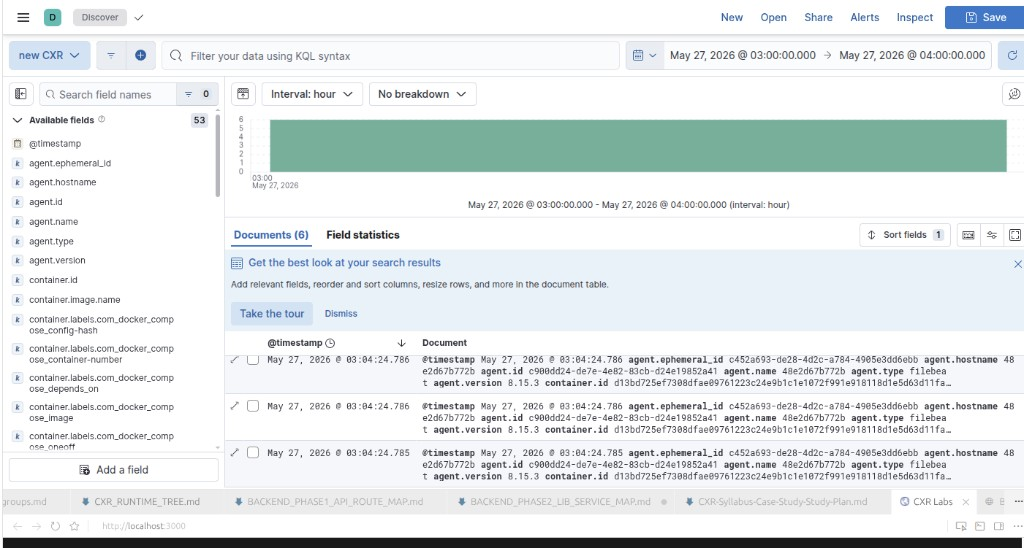
\includegraphics[width=0.92\textwidth]{../evidence/SW12-kibana-discover-2026-05-31.png}
\caption{Kibana Discover --- \texttt{filebeat-*} docs from :3000 \texttt{cxr-ui} (SW.12 evidence).}
\end{figure}

\end{document}
